\documentclass[tikz,border=4pt]{standalone}
% Paleta y fuentes compartidas por el libro y las figuras (única fuente de verdad).
\RequirePackage{xcolor}
\definecolor{oxido}{HTML}{B7410E}
\definecolor{cobre}{HTML}{D27D2D}
\definecolor{carbon}{HTML}{2B2B2B}
\definecolor{azul}{HTML}{1F5F8B}
\definecolor{arena}{HTML}{F4EDE4}

\usepackage{fontspec}
\setsansfont{FiraSans}[Extension=.otf,UprightFont=*-Regular,BoldFont=*-SemiBold,ItalicFont=*-Italic,BoldItalicFont=*-SemiBoldItalic]
\setmonofont{FiraMono}[Extension=.otf,UprightFont=*-Regular,BoldFont=*-Medium,Scale=0.95]
\usetikzlibrary{positioning,arrows.meta,calc,decorations.pathreplacing}
\begin{document}
\sffamily\small
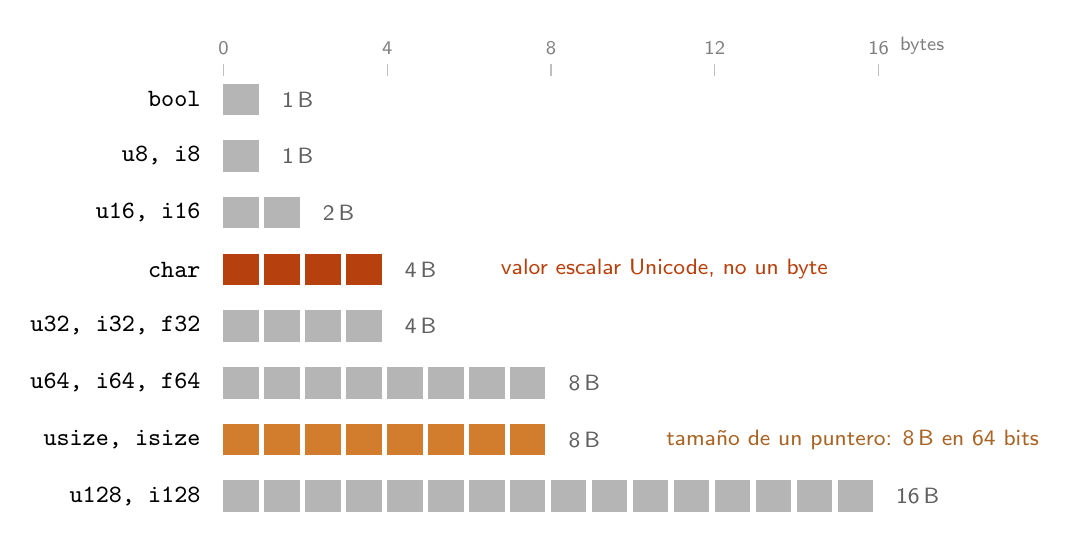
\begin{tikzpicture}[
  tipo/.style={anchor=east,font=\ttfamily\small,inner sep=1pt},
  nota/.style={anchor=west,font=\sffamily\footnotesize,text=carbon!75}]
  \def\b{0.52}  % ancho de un byte
  \def\paso{0.72}
  \foreach \i/\t/\n/\c in {
      0/{bool}/1/carbon!35,
      1/{u8, i8}/1/carbon!35,
      2/{u16, i16}/2/carbon!35,
      3/{char}/4/oxido,
      4/{u32, i32, f32}/4/carbon!35,
      5/{u64, i64, f64}/8/carbon!35,
      6/{usize, isize}/8/cobre,
      7/{u128, i128}/16/carbon!35} {
    \node[tipo] at (-0.25,-\i*\paso) {\t};
    \foreach \k in {1,...,\n} {
      \fill[\c] ({(\k-1)*\b},-\i*\paso-0.2) rectangle ({\k*\b-0.07},-\i*\paso+0.2);}
    \node[nota] at ({\n*\b+0.1},-\i*\paso) {\n\,B};
  }
  % Escala
  \foreach \k in {0,4,8,12,16} {
    \draw[carbon!30] ({\k*\b},0.45) -- ({\k*\b},0.3);
    \node[font=\sffamily\scriptsize,text=carbon!60,anchor=south] at ({\k*\b},0.45) {\k};}
  \node[font=\sffamily\scriptsize,text=carbon!60,anchor=south west] at ({16*\b+0.15},0.45) {bytes};
  % Notas laterales
  \node[nota,text=oxido] at (3.4,-3*\paso) {valor escalar Unicode, no un byte};
  \node[nota,text=cobre!80!black] at (5.5,-6*\paso) {tamaño de un puntero: 8\,B en 64 bits};
\end{tikzpicture}
\end{document}
